\documentclass[notitlepage,12pt]{article}
\usepackage[margin=1in]{geometry}
\usepackage{natbib}
\usepackage{graphicx}
\usepackage{titling}
\usepackage{url}
\graphicspath{{../img/report/}}


\title{%
Interactive Terrain Deformation \\
\large CGI Techniques and ASE Project}
\date{}

\begin{document}
\maketitle

\thispagestyle{empty}

\begin{abstract}
\noindent With GPU processing becoming more and more advanced each year, hundreds of level-of-detail (LOD) approaches have been created to try to tackle displaying terrains in the most efficient way. In this paper, a few different techniques and algorithms will be analysed, and their prose stated, then taking a combination of these techniques, my initial project design will be described. The goal of the project is to provide a tool to load terrain, allow the modification of parts of the terrain, then the ability to output to a file to be used in other VFX programs such as Maya.
\end{abstract}

\newpage
\clearpage
\setcounter{page}{1}

\section{Introduction}
% 100 words

Creating large-scale, realistic, and visually-stimulating terrains is both a time and resource intensive task. Within the visual effects (VFX) industry, it can take huge teams of artists and developers to design and develop these terrains. Having many departments slowly iterating and adapting a design can take many months to suit the desired use-case of the terrain.

With more and more landscapes being created each year, tools that can transform the work of an entire department into the work of a single person are of key interest to VFX houses. The need for hyper-realism in both film and games, and having methods for representing these terrains, and options for modifying and creating new terrain, has become an important area of research within computer graphics. In the current climate, the rise of streaming sites that have a high turnover of shows has become more prevalent, and being able to make these beautiful terrains quickly has become very important to the success of theses platforms \textit{(example of a TV show that uses computer generated terrains: `The Mandalorian', \cite{mandalorian})}.

This is the area of computer graphics that my project shall address. I shall identify and analyse some existing tools and algorithms that currently exist, merit and critique each source, then finally describe what my project will do.

\section{Literature Review}
% 1200 words

\subsection{Quadtrees and Octrees}

\begin{figure}[ht]
  \centering
  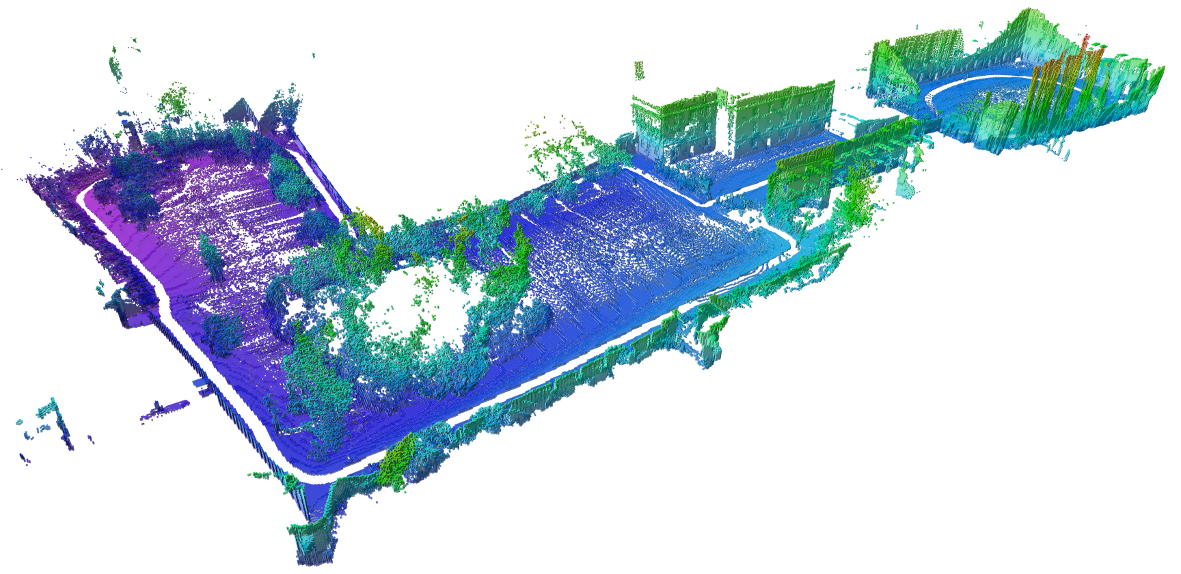
\includegraphics[width=1.0\textwidth]{octomap.png}
  \caption{An example of the ``blocky'' nature of the terrain when stored in octrees. \textit{Credit \cite{octrees}}}
  \label{fig:octrees}
\end{figure}

Quadtrees and octrees utilise tree-like data structures to represent large sizes of data in efficient compressed formats. Quadtrees are good for representing 2D data with octrees being better suited for 3D representation. In these tree structures, each node only has children if the data cannot be represented by this single node, \cite{quadtreesOctrees}. 

Using these data structures, large terrains can be represented in efficient ways that are easier to compute and send to the GPU, than the full size objects. As sending data between the CPU and GPU are the main bottlenecks in these systems, requiring the transfer of a small amount of data (that represents lots of information), makes these trees useful for terrain representation.

Octrees are frequently used for LOD systems due to their inherent ability to represent 3D terrains, \cite{lod}. One example of their use is in 3D mapping for drone systems. 

In \cite{octrees}, octrees are used to store volumetric, 3D environment models to help drones navigate the terrain. Accurate 3D models of the terrain can be taken and stored efficiently, with any gaps being probabilistically estimated. This quick-running algorithm works perfectly in the real-time system of automated drone flying. Unfortunately, very complex terrain needs detailed octrees to represent it correctly otherwise the terrain can look ``blocky'' or low quality (see figure \ref{fig:octrees}).

Although octrees are more commonly used, quadtrees can also be adapted for terrain representation. In \cite{quadtrees}, a two-step, surface simplification process is introduced to decide the LOD level for each block of triangles. The first step is using a coarse-grained simplification algorithm to determine the LOD levels required for that block. The second step is a fine-grained retriangulation of each block where individual vertices are compared with the original data and considered whether they are required or not to represent the data accurately in this quadtree-like structure.

Whilst the algorithm described here suitably provides a real-time solution, the complexity of the implementation, and the lack of ability to modify the data during runtime, makes this solution unsuitable for my project.

\subsection{Real-time Optimally Adapting Mesh (ROAM)}

\begin{figure}[h]
  \centering
  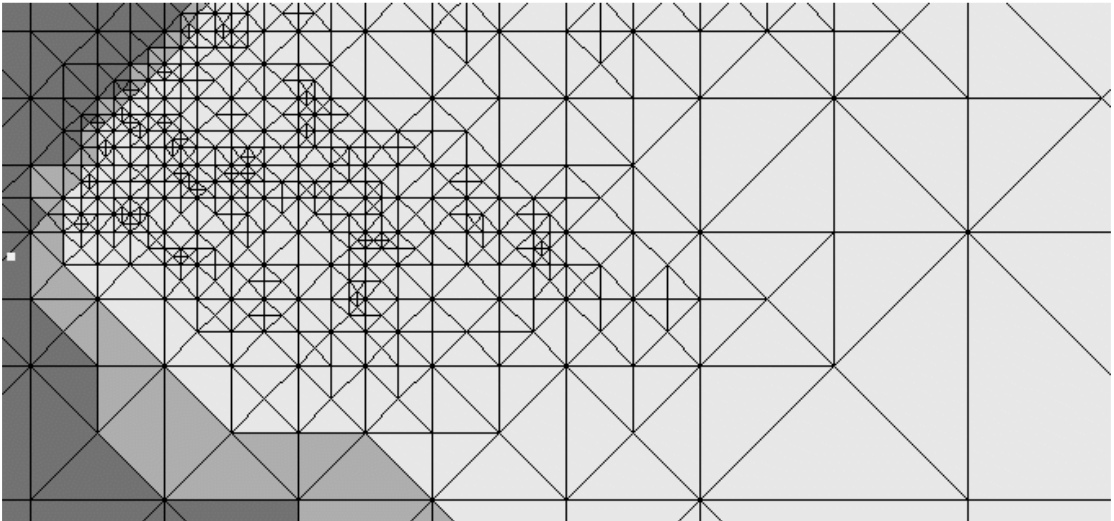
\includegraphics[width=1.0\textwidth]{roam.png}
  \caption{An example of the triangulation of the terrain in the ROAM algorithm. \textit{Credit \cite{roam}}}
  \label{fig:roam}
\end{figure}

Another type of tree structure that can be used in terrain representation is a bintree. In the ROAM algorithm, using some sophisticated approaches, they are able to achieve high frame-rates when displaying thousands of triangles, \cite{roam}. 

Meshes are defined as a bintree of triangles, wherein each node represents the triangles of its two children but in a coarser LOD (see figure \ref{fig:roam}). The important details are determined, and using the view-distance parameter, this information is passed on to traditional LOD algorithms. As ROAM works on a per triangle basis, it reduces any ``popping'' of LOD levels and also helps to solve the massive mesh problem (where large portions need to be loaded at a time to determine LOD level for the whole section).

Unfortunately, ROAM doesn't work well on the GPU. This is due to data needing to constantly be re-uploaded which can result in ``thrashing'' the GPU, stalling it as it waits for the data to be written. Therefore, ROAM is better suited to rendering for film, instead of its use in video games that require real-time rendering.

One solution to this is to keep the vertex buffer static and only change the index buffer based on the current LOD. This is what \cite{roamGeomancy} does to make ROAM better suited to video games. Whilst this works well and provides real-time rendering, the terrain represented is restricted to terrains with uniform X-Z spacing of vertices--an issue that is prevalent with many terrain algorithms.

\subsection{Geomipmapping}

To avoid having to represent the entire terrain's X-Z coordinates, geomipmapping works by splitting the terrain into equally sized chunks with uniform X-Z coordinates that can be duplicated and placed all over the terrain. In \cite{geomipmapping}, sets of meshes are represented by blocks of vertices, and then depending on the LOD level, will be skipped to reduce the triangle count. Some of the failings of this original algorithm is the amount of data that needs to be sent between the CPU and GPU, and the problem with stitching two different LOD levels together.

In \cite{geomipmappingScape}, there are three types of buffers used; A vertex buffer for X-Z vertices in a chunk, another for all the Y coordinates of the terrain, and an index buffer for each LOD level that describes which vertices to use. The LOD level of each chunk is dependent on the LOD levels of the neighbouring chunks, and most of the complex calculations are computed on the GPU to reduce the data sent between the CPU and GPU. This algorithm also fixes the stitching problem by having predefined ways of stitching each LOD level together. The main failing of this solution is its complexity as the maths to calculate the stitching is complex and time consuming to work out. This is where the simpler and better approach of geoclipmapping comes in.

\subsection{Geoclipmapping} \label{geoclipmap}

\begin{figure}[h]
  \centering
  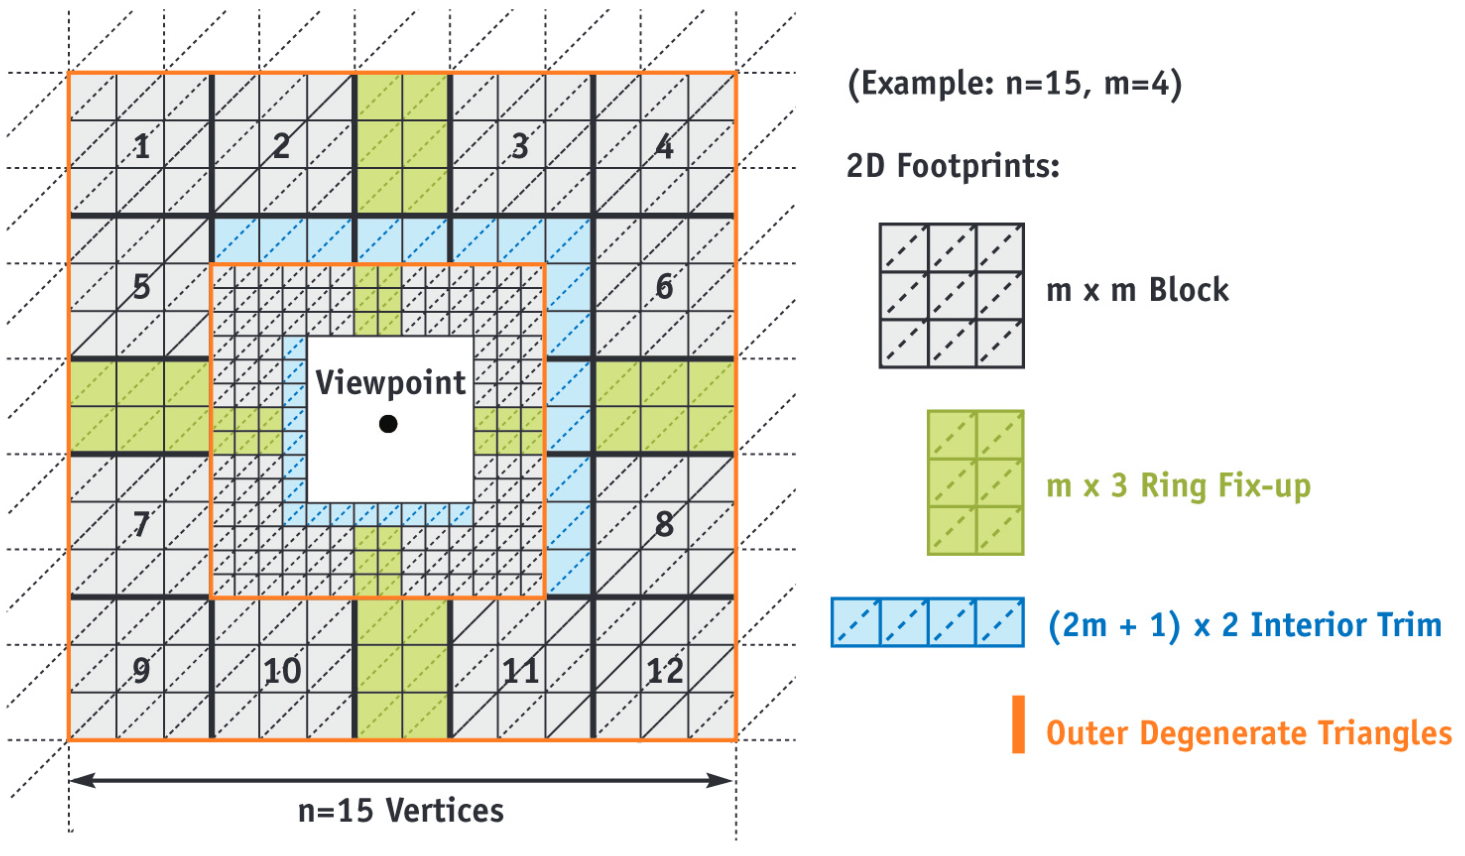
\includegraphics[width=1.0\textwidth]{geoclipmapping_footprints.png}
  \caption{An example of geoclipmapping and the 2D footprints that make up each clipmap. \textit{Credit \cite{geoclipmappingGPUGems}}}
  \label{fig:geoclipmapping}
\end{figure}

In geoclipmapping, just like geomipmapping, X-Z coordinates are represented by a few vertices and indices, with terrain data being cached in a set of nested grids centred around the viewer. Each grid is stored as a constant vertex buffer made up of four different ``footprints'' (see figure \ref{fig:geoclipmapping}) in video memory, whilst the height data is stored as a texture to be read in the vertex shader. The original paper to describe geoclipmapping was \cite{geoclipmapping}, with one of the authors later working alongside NVIDIA to create a chapter for GPU Gems 2, \cite{geoclipmappingGPUGems}.

The main algorithm works by filtering the terrain into a power-of-two mipmap pyramid, with the mipmap being rendered at each pixel being a function of screen-space and parametric derivatives based on the view parameters, not the actual content of the image. The texture clipmap is then updated in fast incremental stages allowing massive landscapes to be traversed with no drop in frames. The LOD level for each clipmap is selected based on the viewer distance. This makes every triangle the same amount of pixels on screen, as each clipmap is just the finest clipmap but at power-of-two scales.

Geoclipmaps have several advantages over other LOD methods. These advantages include the simplicity to implement, having an optimal rendering throughput, retaining visual continuity across clipmaps, and providing complexity throttling that prevents GPU throttling. This works by rendering from the coarsest detail to finest, dropping the finest level if the viewer has moved before rendering.

\subsection{Modification and Procedural Content Generation (PCG)} \label{pcg}

As my project is a fusion of representation algorithms and procedural modification, some research into PCG methods and their uses in terrain has also been carried out. The main problem that is to be solved is trying to create realistic terrain in a computationally inexpensive way.

When trying to create realistic-looking terrain, algorithms that are derived from nature and then simplified into an approximation of the real-world processes can be used to achieve terrains that are indistinguishable from the real thing. Simply creating high and low points at random using basic algorithms like Perlin noise can create these desired effects, \cite{perlin}. However, better results have been seen from water erosion algorithms as seen in \cite{hydrology}.

In the first algorithm, Perlin noise has been effectively used, alongside feature constraints, to create realistic ridge lines, cliff faces, and riverbeds, whilst running efficiently on the GPU. 

In the second, iterative generation using graphs made from the underlying terrain is executed to create complex drainage networks that simulate water erosion across a landscape. The results of these algorithms are hyper-realistic, making them paramount research for terrain generation.

\section{Project Specification}
% 500 words

This project can be split into two sections; The representation of the terrain and the modification/creation of new parts of the terrain. The section that is most important to get right is the representation of the terrain. This is because being able to represent massive terrains efficiently is a key goal of this project.

The algorithms dealing with the representation of the terrain will follow the geoclipmapping algorithms outlined in section \ref{geoclipmap}, and also take influences from the other algorithms I described. 

The high-level overview of this section is as follows; An X-Z vertex buffer will be generated for each footprint of the clipmap, with a corresponding index buffer, and this will be buffered to the GPU for each of the clipmap levels. The height values (that will initially come from a loaded in heightmap) will be buffered to a terrain buffer, read in the vertex shader, then combined with the X-Z values to create a vertex in world space. Methods to blend LOD regions together will be used to avoid any holes in the terrain (see figure \ref{fig:blending}).

\begin{figure}[h]
  \centering
  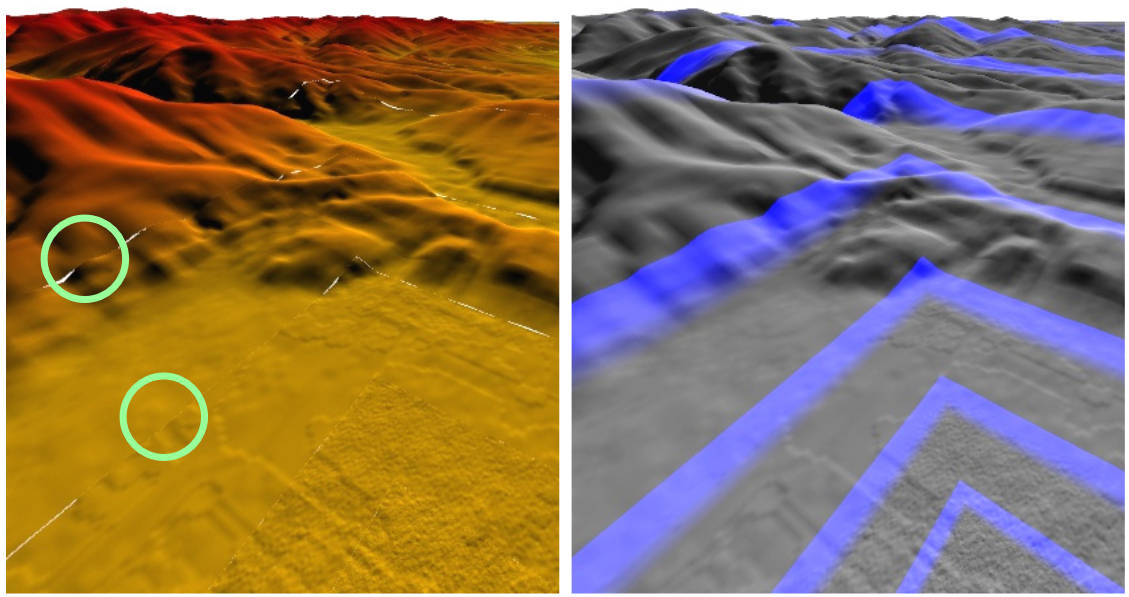
\includegraphics[width=1.0\textwidth]{blen_regions_and_gaps.png}
  \caption{An example of the gaps that need to be blended in geoclipmapping between clipmap levels. \textit{Credit \cite{geoclipmapping}}}
  \label{fig:blending}
\end{figure}

The world will be centred around the viewer and clipmap levels will be generated based on this location. The world will seemingly be an infinite flat world, with the loaded-in heightmap occupying the area around the origin. Regions of this world can be saved to object files that can be read by Maya or equivalent modelling software to be used in film or games.

Once the representation section is fully developed, work on the modification algorithms can begin. 

Here, different types of brushes and tools will be available as part of a UI that allow the user to modify the terrain in interesting ways to suit their needs. Some of the tools will be quite simple in nature--merely modifying the heights and colours of the terrain at certain locations. The complexity of this section is in the PCG tools that will be made available. These tools will use algorithms described in section \ref{pcg} to help build highly detailed scenery, that can be exported to object files for use in other software.

Due to my limited (but growing) knowledge in the area of computer graphics, I am leaving the PCG tools until last, where they will only be implemented if time permits. The main goal will be to have a working tool that can load heightmaps, allow basic modifications, then save to the desired object file. Any extra time can then be spent on the PCG tools that will require a decent level of understanding in the area (which will hopefully come as the project develops).

\section{Conclusion}
% 200 words

Many algorithms for representing and displaying terrain have been developed since the start of the computer graphics epoch, with some taking inspiration from traditional data structures, and others coming up with novel ones that are sometimes more efficient, but often more complicated to implement.

I have highlighted the algorithms that I intend to take notes from when developing my project, briefly explaining the algorithm, and critiquing the approach. A wide variety of existing solutions have been discussed here--each with their own advantages and disadvantages--giving an extensive overview of the topic area at present. 

Based on the advantages and disadvantages of the existing algorithms, I have opted for a mix of most of them, with the main algorithm taking inspiration from geoclipmapping (section \ref{geoclipmap}). This algorithm seems the easiest to implement with significant benefits to efficiency compared with the other solutions.

However, some issues with this approach may be encountered, mostly due to my developing knowledge of computer graphics. To counteract this, I have tried to split and simplify the project, whilst describing the milestones I will try to reach for each section, in the given time-frame.

The success criteria were touched on, with the functional requirement of the project being the ability to load and save the terrain, and the non-functional requirements of having constant framerates and low memory usage being important to the project's success.

Finally, when my project is finished, I can compare it to some existing solutions to deem whether my project has been an overall success.

\clearpage
\bibliographystyle{agsm}
\bibliography{report}

\end{document}